\documentclass[12pt]{scrartcl}                                                      % 'Artikel' Dokumentenklasse und Standardschriftgröße  
\usepackage[paper=a4paper,left=2.5cm,right=2.5cm,top=2.5cm,bottom=2.5cm]{geometry}  % Setzt das Papierformat und den Rand auf 2.5cm

\setlength{\parindent}{0mm}                                                         % Setzt die Einrückung von Absätzen auf gegebenen Abstand

\usepackage[T1]{fontenc}                                                            % Legt FontKodierung fest
\usepackage[utf8]{inputenc}                                                         % Legt Zeichenkodierung fest

\usepackage[ngerman]{babel}                                                         % Deutsche Rechtschreibung
\usepackage[ngerman]{varioref}                                                      % Versieht Referenzen mit Bezeichnung des Objektes
%\usepackage{lmodern}                                                                % Empfohlener T1-Font für deutsche Texte

%%%%%%%%%%%%%%%%%%%%%%%%%%%%%%%%%%%%%%%%%%%%%%%%%%%%%%%%%%%%%%%%%%%%%%%%%%

\usepackage{fancyhdr}                                                               % Ermöglicht detailierte Bearbeitung der Kopf- und Fußzeile
\fancyhf{} 	                                                                        % Setzt Kopf und Fußzeile zurück 
\setlength{\headheight}{28.0pt}                                                     % Höhe der Kopfzeile
\setlength{\footskip}{18.0pt}                                                       % Höhe der Fußzeile

\renewcommand{\headrulewidth}{.5pt}                                                 % Dicke des Kopfzeilentrennstrichs
\renewcommand{\footrulewidth}{.5pt}                                                 % Dicke des Fußzeilentrennstrichs

\lhead{\textbf{\VNr\ \VN}}                                                                   % Angabe Links-Oben
%\chead{}                                                                           % Angabe Mitte-Oben
\rhead{\VD}                                                                      % Angabe Rechts-Oben
%\lfoot{}                                                                           % Angabe Links-Unten
\cfoot{\textbf{\thepage\ von \pageref{LastPage}}}                                   % Angabe Mitte-Unten
\rfoot{Johannes Schlüter\\ Joshua Luckey}                                           % Angabe Rechts-Unten

%%%%%%%%%%%%%%%%%%%%%%%%%%%%%%%%%%%%%%%%%%%%%%%%%%%%%%%%%%%%%%%%%%%%%%%%%%
\usepackage{scrdate}
\usepackage{lastpage}                                                               % Macht die letzte Seitenzahl referenzierbar mit \pageref{Lastpage}
%\usepackage{natbib}                                                                % Bessere BibTeX-Einträge
%\usepackage{hyperref}                                                              % Ermöglicht Verlinkungen im Dokument

%%%%%%%%%%%%%%%%%%%%%%%%%%%%%%%%%%%%%%%%%%%%%%%%%%%%%%%%%%%%%%%%%%%%%%%%%%

\usepackage[sumlimits,intlimits,namelimits]{amsmath}                                % Fügt mathematische Symbole hinzu, setzt Grenzen, Limiten und Indizes unter das Symbol und nicht dahinter
\usepackage{amssymb}                                                                % Fügt Symbole wie z.B. Zahlenmengen wie $\mathbb{R}$ hinzu 
\usepackage{amsthm}                                                                 
\usepackage{amsfonts}                                                               % Fügt Font für Mathematikumgebung hinzu

\usepackage{empheq}                                                                 % Stellt verbesserte Gleichungsumgebung bereit \begin{empheq}[<Aussehen>]{<Umgebungstyp>} ... \end{empheq}
%test
%\usepackage[version=3]{mhchem}                                                     % Stellt chemische Struktur und Summenformeln bereit \ce{<Summenformel>}
%\usepackage{chemfig}                                                               % Stellt chemische Valenzstrichformeln fürganze Moleküle bereit \chemfig{<Molekül-Aufbau>}

\usepackage{siunitx}                                                                % Stellt eine verbesserte Formatierung von größen mit Einheiten zur Verfügung  
\sisetup{locale = DE,prefixes-as-symbols = false}                                   % Setzt das 'Mal'-Zeichen auf \cdot und das Dezimaltrennzeichen auf ',' 
                                                                                    % und ersetzt Prefixe wie '\kilo' mit der entsprechenden Zehnerpotenz
\sisetup{separate-uncertainty = true}                                               % Ermöglicht vereinfachtes eintragen von Unsicherheiten '42.6(4)' --> '42.6 +/- 0.4'                                                                                 

\usepackage{textcomp}                                                               % Fügt extra Symbole hinzu   
\usepackage[b]{esvect}                                                              % Fügt verbesserte Vektorpfeile hinzu \vv{<Vektorname>} 

%%%%%%%%%%%%%%%%%%%%%%%%%%%%%%%%%%%%%%%%%%%%%%%%%%%%%%%%%%%%%%%%%%%%%%%%%%

\usepackage{graphicx}                                                               % Ermöglicht das Einbinden Grafiken '\includegraphics[<Optionen>]{<Grafikpfad>}' und Veränderungen im Text, wie z.B. Schriftfarbe 
\usepackage[rflt]{floatflt}                                                         % Fügt Möglichkeit für text umflossende Grafiken und Tabellen hinzu \begin{floating<figure/table>}[option]{width} ... \caption ... \end{floatingfigure}
%\usepackage{subfig}                                                                % Ermöglicht das Hinzufügen von Unterabbildung zu einer Abbildung

\usepackage{tikz}                                                                   % Ermöglicht Zeichnungen im Dokument \begin{tikzpicture} ... \end{tikzpicture}
\usetikzlibrary{arrows}                                                             % Fügt zusätzlichen Pfeilspitzen hinzu
%%%%%%%%%%%%%%%%%%%%%%%%%%%%%%%%%%%%%%%%%%%%%%%%%%%%%%%%%%%%%%%%%%%%%%%%%%

\usepackage[normalem]{ulem}                                                         % Fügt verbesserte Unterschtreichungen hinzu, z.B. doppelt, gezackt, gewellt, etc.
\usepackage{enumitem}                                                               % Ermöglicht detailierte Einstellungen an Aufzählungssymbolen
%\usepackage{slashbox}                                                              % Ermöglicht das Einfügen mehrerer Einträge in eine Tabellenzelle, getrennt von einem '\' \backslashbox{<Eintrag unten-links>}{<Eintrag oben-rechts>} TIPP: Leerzeichen

%%%%%%%%%%%%%%%%%%%%%%%%%%%%%%%%%%%%%%%%%%%%%%%%%%%%%%%%%%%%%%%%%%%%%%%%%%

\title{} 
\author{} 

%%%%%%%%%%%%%%%%%%%%%%%%%%%%%%%%%%%%%%%%%%%%%%%%%%%%%%%%%%%%%%%%%%%%%%%%%%

\pagestyle{fancy}                                                                   % Anwenden des Erweiterten Seitenlayouts

%\renewcommand{\thefootnote}{}
%\setlength{\footnotesep}{2cm}
\setlength{\skip\footins}{2cm}
%\setlength{\itemsep}{7.5pt}


\newcommand{\intd}[1]{\,\mathrm{d}#1}
\newcommand{\im}{\ensuremath{\textsl{i}}}
\newcommand{\e}{\ensuremath{\textsl{e\;\!}}}
%%%%%%%%%%%%%%%%%%%%%%%%%%%%%%%%%%%%%%%%%%%%%%%%%%%%%%%%%%%%%%%%%%%%%%%%%%

\newcommand{\VNr}{V102}                                                             % Makro für die aktuelle Versuchsnummer
\newcommand{\VN}{Drehschwingungen}                                                  % Makro für den aktuellen Versuchsnamen
\newcommand{\VD}{31. Oktober 2013}                                                  % Makro für das Versuchsdatum


\begin{document}

  \section{Einleitung}
    Im Versuch Drehschwingungen V102 sind verschiedene Messungen durchzuführen und mit Hilfe 
    derer die elastischen Konstanten eines Material zu bestimmen. Hierbei kann eine beliebige Metalllegierung 
    untersucht werden - In diesem Fall ein Kupferdraht. 
    Außerdem wird in einem zweiten Messgang noch das magnetische Moment eines Magneten durch 
    Drehschwingungen unter Einfluss eines homogenen Magnetfeldes, welches mit Hilfe von Helmholtzspulen erzeugt wird, untersucht.


  
  
  %\section{Aufgaben}
  
  
  
    %\subsection{Vorbereitungsaufgaben}
    
    
    
    %\subsection{Augabenstellung}
    
    
    
  \section{Theorie}
    Bei den im erseten Versuchsteil zu bestimmenden Größen, handelt es sich um sogenannte \emph{elastische Konstanten},
    die im allgemeinen ein Maß für die relative Form- und Volumenveränderung eines Materials sind, welches äußeren Kräften
    ausgesetzt ist. Solche Kräfte die auf die Oberfläche eines Matrials einwirken wie beispielsweise der Druck, werden
    im allgemeinen Spannungen genannt. Die Anzahl der zur Beschreibung eines Materials nötigen elastischen Konstanten, 
    hängt vorallem von der inneren Struktur des Materials ab und reicht von einem Maximum von $36$ Konstanten zu einem
    Minimum von $2$ Konstanten für isotrope Materialien wie sie auch in diesm Versuch untersucht werden.
    Zu den zwei benötigten Konstanten, dem Torsionsmodul $G$ und dem Kompressionsmodul $Q$ kommen in diesem Versuch
    noch zwei weitere, das Elastizitätsmodul $E$ und die Poissonsche Querkontraktionszahl $\mu$ hinzu.
    Der Zusammenhang dieser vier Größen lässt mit den Gleichungen \ref{EG} und \ref{EQ} beschreiben.
    
    \begin{empheq}{align}
      E &= 2G(\mu + 1)\label{EG} \\
      E &= 3Q(1 - 2\mu) \label{EQ}
    \end{empheq}
    
    
    Die Bestimmung des Torsionsmoduls erflogt in diesem Versuch mit Hilfe einer dynamischen Methode, d.h. die 
    auf den hier zu untersuchenden Draht wirken periodisch zeitabhängige Spannungen. Dies ist der statischen
    Methode gegenüber vorteilhafter, da keine elastischen Nachwirkungen auftreten, durch die das Material 
    nur verzögert in seinen Ausgangszustand zurück geht.
    Für die hier verwendete dynamische Methode, wird der zu untersuchende Draht in harmonische Drehschwingungen
    Mit der Periodendauert
    \begin{empheq}{equation}
      T = \sqrt{\frac{J}{D}} 
      \label{T}
    \end{empheq}
    versetzt. Dabei ist $J$ das Trägheitsmoment des schwingenden Körpers und $D$ die Richtgröße des als
    Zylinder idealisierten Drahtes, welche durch Gleichung \ref{D} beschrieben wird.
    \begin{empheq}{equation}
      D = \frac{\pi G R^{4}}{2L}
      \label{D}
    \end{empheq} 
    
    Für die Bestimmung des magentischen Moments $m$ im zweiten Versuchsteil wird die durch
    
    \begin{empheq}{equation}
      B = \mu_{0}\mu_{r}\frac{8}{\sqrt{125}}\frac{IN}{R}\cite{Test} 
      \label{B}
    \end{empheq}
    
    berechenbare magnetische Flussdichte eines Helmholtzspulenpaares benötigt, für die somit
    die geometrischen Abmessungen der Spulen  und der durch diese fließende Strom $I$ benötigt werden.
    Auch in diesem Versuchsteil wird der Daht in harmonische Schwingungen versetzt deren Periodendauer
    \begin{empheq}{equation}
      T_{m} = \sqrt{\frac{J}{mB + D}} 
      \label{T}
    \end{empheq}
    ist.
    
    
  \section{Durchführung}
  
    Der Versuchsaufbau entspricht dem in Abbildung \ref{Aufbau} mit dem Zusatz, dass links von der Apparatur 
    noch eine Glühlampe mit Blende und Fokussierlinse steht und um etwa 90° versetzt ein 
    Photodiode, welcher ein H-Signal weitergibt, wenn diese von dem Lichtstrahl über den Spiegel 
    getroffen wird.
    Als erstes ist gefordert eine Stoppuhr mit einer Logikschaltung selber zu erstellen, diese soll 4 
    Phasen haben:
    
    \begin{enumerate}
      \item{Start der Stoppuhr} 
      \item{\glqq Nichts\grqq\ } 
      \item{Stopp der Stoppuhr} 
      \item{Reset der Stoppuhr} 
    \end{enumerate}
    
    Sobald der Lichtstrahl vom Spiegel reflektiert wird und dieser in die Photodiode trifft, gibt 
    diese ein Signal auf die Schaltung, dann geht die Stoppuhr in Phase 1, beim zweiten Mal in 
    Phase 2 usw..
    Danach wird noch die Dicke des Drahtes an 4 verschiedenen Stellen vermessen und 
    andere feste Größen an der Apparatur abgelesen.
    
    Durch das Justierrad mit Klemmschraube wird der Spiegel so ausgerichtet, dass der 
    Lichtstrahl neben der Photodiode auf der dort justierten Mattscheibe zu sehen ist, danach wird 
    eine Auslenkung durch  
    das Justierrad erzeugt und die Periodendauern von der Stoppuhr abgelesen und notiert bis 
    eine ausreichende Menge an Messwerten vorhanden ist.  
    Schlussendlich werden nun die Helmholtzspulen eingeschaltet, damit ein homogenes 
    Magnetfeld erzeugt wird, um dann die Messungen noch einmal auszuführen.
    \begin{figure}[B]
      \centering
      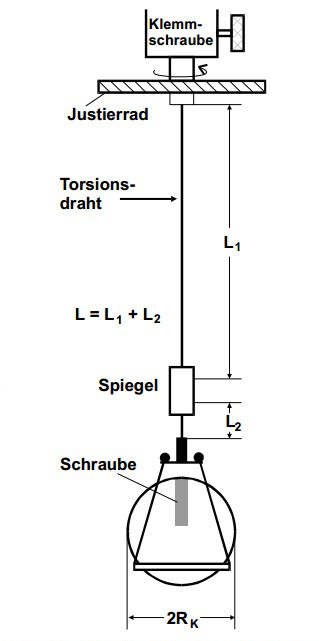
\includegraphics[scale = 0.65]{Grafik/Versuchsaufbau.jpg}%
      \caption{Skizze des Versuchsaufbaus}
      \label{Aufbau}%
    \end{figure}
    
  
  
  \section{Auswertung}
    Im folgenden sind die aufgenommenen Messwerte, sowie die aus diesen berechneten Werte
    aufgeführt. An entsprechenden Stellen sind Erläuterungen zu den Berechnungen gegeben.
    Der nachflogenden Abschnitt \ref{Fehlerrechnung} enthält die Fehlergleichungen für die hier
    aufgeführten Größen.
    
    In den Tabellen \ref{Draht} bis \ref{Spule} sind für die noch folgenden Rechnungen benötigten
    Apparaturgößen angegeben.
    
      \begin{table}% Drahtdaten
        \begin{tabular}{|C|C|}
          \hline
          Durchmesser & Länge \\
          $d[\si{mm}]$ & $L[\si{cm}]$\\ \hline\hline
        
        \end{tabular}
        \caption{Messgrößen des Drahtes}
        \label{Draht}
      \end{table} 
      
      \begin{table}% Kugeldaten
        \begin{tabular}{|C|C|C|}
          \hline
          Masse & Durchmesser & Trägheitsmoment\\
          $m_{K}[\si{g}]$ & $d_{K}[\si{cm}]$ &der Halterung \\ 
            512.50(4)         &                            & $I_{H}[\si{gcm^{2}}]$ \\ \hline \hline
          
                          
        
        \end{tabular}
        \caption{Messgrößen der Kugel und Halterung}
        \label{Kugel}
      \end{table} 
      
      
      \begin{table}% Spulendaten
        \begin{tabular}{|C|C|}
          \hline
          Radius $R[\si{mm}]$  & Windungszahl $N$\\ \hline\hline
          78.0         & 390        \\ 
          \hline
        \end{tabular}
        \caption{Messgrößen der Spulen}
        \label{Spule}
      \end{table}
      

  

    
    
      \begin{table}[h]
        \begin{tabular}{|C||C|}
          \hline
          Periodendauer & Periodendauer \\ 
          $T[\si{\second}]$ & $T[\si{\second}]$\\
          \hline \hline
          \num{18,364(1)} & \num{18,330(1)}\\ 
          \num{18,377(1)} & \num{18,333(1)}\\ 
          \num{18,353(1)} & \num{18,343(1)}\\ 
          \num{18,359(1)} & \num{18,320(1)}\\ 
          \num{18,346(1)} & \num{18,342(1)}\\ \cline{2-2}   
          \num{18,349(1)} & $\overline{T} = \num{18.3469(3)}$ \\ \hline
    
    
        \end{tabular}
        \centering
        \caption{Gemessene Periodendauern ohne äußeres Magnetfeld}
        \label{Tab1}
      \end{table}
      

  \subsection{Fehlerrechnung}
    \label{Fehlerrechnung}
  $\sqrt{0.16 \sigma_{m_{K}}^{2} r_{K}^{4} + 0.64 \sigma_{r_{K}}^{2} m_{K}^{2} r_{K}^{2}}$
  
  $\displaystyle \sqrt{\frac{64 \pi^{2} L^{2} \sigma_{I_{K}}^{2}}{R^{8} T^{4}} + \frac{256 \pi^{2} L^{2} \sigma_{T}^{2}}{R^{8} T^{6}} \left(I_{H} + I_{K}\right)^{2} +
  \frac{1024 \pi^{2} L^{2} \sigma_{R}^{2}}{R^{10} T^{4}} \left(I_{H} + I_{K}\right)^{2} + \frac{64 \pi^{2} \sigma_{L}^{2}}{R^{8} T^{4}} \left(I_{H} + I_{K}\right)^{2}}$
  
  $\displaystyle  \sqrt{\frac{E^{2} \sigma_{G}^{2}}{4 G^{4}} + \frac{\sigma_{E}^{2}}{4 G^{2}}}$
  
  $\displaystyle  \sqrt{\frac{36 E^{2} \sigma_{\mu}^{2}}{\left(- 6 \mu + 3\right)^{4}} + \frac{\sigma_{E}^{2}}{\left(- 6 \mu + 3\right)^{2}}}$
  
  $\displaystyle  \sqrt{\frac{I^{2} N^{2}}{R^{4}} \frac{64}{125}\mu_{0}^{2} \sigma_{R}^{2} + \frac{I^{2} \sigma_{N}^{2}}{R^{2}}\frac{64}{125}\mu_{0}^{2}+ \frac{N^{2} \sigma_{I}^{2}}{R^{2}} \frac{64}{125}\mu_{0}^{2}}$
  \section{Diskussion}
   
  $ \sqrt{\sigma_{B}^{2} \left(\frac{\pi G R^{4}}{2 B^{2} L} - \frac{ 4\pi^{2} }{B^{2} T^{2}} \left(I_{H} + I_{K}\right)\right)^{2} + \frac{4\pi^{2} G^{2} R^{6} \sigma_{R}^{2}}{B^{2} L^{2}} + \frac{\pi^{2} G^{2} R^{8} \sigma_{L}^{2}}{4 B^{2} L^{4}} + \frac{16\pi^{4} \sigma_{I_{K}}^{2}}{B^{2} T^{4}} + \frac{16 \pi^{2} \sigma_{T}^{2}}{B^{2} T^{6}} \left(I_{H} + I_{K}\right)^{2} + \frac{\pi^{2} R^{8} \sigma_{G}^{2}}{4 B^{2} L^{2}}}$

\end{document}

